%
%===============>>  Сорокин Модуль 7 <<=============
%
\setmodule{7}

%BEGIN_FOLD % ====>>_____ Занятие 1 _____<<====
\begin{class}[number=1]
	\begin{listofex}
		\item В треугольнике \( ABC \) \( AD \)  — биссектриса, угол \( C \) равен \( 50^{\circ} \), угол \( CAD \) равен \( 28^{\circ} \). Найдите угол \( B \). Ответ дайте в градусах.
		\item В остроугольном треугольнике \( ABC \) угол \( A \) равен \( 65^{\circ} \). \( BD \) и \( CE \)  — высоты, пересекающиеся в точке \( O \). Найдите угол \( DOE \). Ответ дайте в градусах.
		\item В треугольнике \( ABC \) проведена биссектриса \( AD \) и \( AB = AD = CD \). Найдите меньший угол треугольника \( ABC \). Ответ дайте в градусах.
		\item Один из углов треугольника в \( 2 \) раза больше второго, а третий угол равен \(  33^{\circ} \). Определите два неизвестных угла треугольника.
		\item
		\begin{minipage}[t]{\bodywidth}
			Найдите угол \( \alpha \) (если на чертеже необходимо выделить четыре или более углов, то их отмечают одной дугой).
		\end{minipage}
		\hspace{0.02\linewidth}
		\begin{minipage}[t]{\picwidth}
			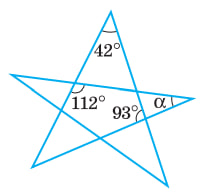
\includegraphics[align=t, width=0.8\linewidth]{../../../../../exercises/lists/pics/sorokinM7L1-2}
		\end{minipage}
		\item В треугольнике \( ABC \) углы \( A \) и \( C \) равны \( 20^{\circ } \) и \( 60^{\circ} \) соответственно. Найдите угол между высотой \( BH \) и биссектрисой \( BD \). 
		\item В треугольнике \( ABC \) угол \( A \) равен \( 30^{\circ} \), угол \( B \)  — тупой, \( CH \)  — высота, угол \( BCH  \) равен \( 22^{\circ} \). Найдите угол \( ACB \). Ответ дайте в градусах.
	\end{listofex}
\end{class}
%END_FOLD

%BEGIN_FOLD % ====>>_ Домашняя работа 1 _<<====
\begin{homework}[number=1]
	\begin{listofex}
		
		\item В прямоугольном треугольнике угол между высотой и медианой, проведенными из вершины прямого угла, равен \( 40^{\circ} \). Найдите больший из острых углов этого треугольника.
		\item В треугольнике \( ABC \) углы \( A \) и \( C \) равны \( 30^{\circ} \) и \( 50^{\circ} \) соответственно. Найдите угол между высотой \( BH \) и биссектрисой \( BD \).
		\item В треугольнике \( ABC \) угол \( A \) равен \( 38^{\circ} \), угол \( B \) - тупой, \( CH \)  — высота, угол \( BCH \) равен \( 35^{\circ} \). Найдите угол \( ACB \). Ответ дайте в градусах.
		\item В треугольнике \( ABC \) угол \(  A \) равен \( 7^{\circ} \), внешний угол при вершине \( B \) равен \( 22^{\circ} \). Найдите угол \( C \).
	\end{listofex}
\end{homework}
%END_FOLD

%BEGIN_FOLD % ====>>_____ Занятие 2 _____<<====
\begin{class}[number=2]
	\begin{listofex}
		\item Один из углов треугольника в \( 4 \) раза больше третьего, а второй угол угол равен \(  25^{\circ} \). Определите два неизвестных угла треугольника.
		\item 
		\begin{minipage}[t]{\bodywidth}
			В треугольнике \( ABC \)  \( AB = BC \), \( BAD=105\degree \). Найдите угол \( MCN \).
		\end{minipage}
		\hspace{0.02\linewidth}
		\begin{minipage}[t]{\picwidth}
			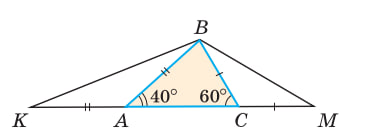
\includegraphics[align=t, width=1.3\linewidth]{../../../../../exercises/lists/pics/sorokinM7L2-1}
		\end{minipage} 
		\item 
		\begin{minipage}[t]{\bodywidth}
			В треугольнике \( ABC \) \( \angle A = 40^{\circ} \), \( 
			\angle C = 60^{\circ} \), \( AK = AB \), \( CM = CB \). Найдите угол \( KBM \).
		\end{minipage}
		\hspace{0.02\linewidth}
		\begin{minipage}[t]{\picwidth}
			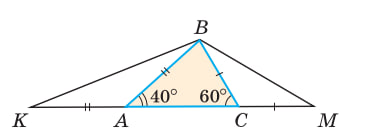
\includegraphics[align=t, width=1.3\linewidth]{../../../../../exercises/lists/pics/sorokinM7L1-1}
		\end{minipage} 
		\item Известно, что  \( \angle BAC = 68\degree \), \( AM \) — биссектриса угла \( BAC \),\( AK \) — биссектриса угла \(  MAC \). Найдите градусную меру угла \( BAK \).
		\item После того как один из смежных углов увеличили на \( 40\% \), другой угол уменьшился на \( 60 \% \). Найдите, какими были по величине первоначально два данных смежных угла.
		\item Углы треугольника относятся как \(  2:8:35 \). Найдите меньший из них. Ответ дайте в градусах.
		\item Углы треугольника относятся как \( 2:3:4 \). Найдите отношение соответствующих внешних углов треугольника,
		взятых по одному при каждой вершине.
		\item Два угла треугольника равны \( 58^{\circ} \) и \( 72^{\circ} \). Найдите тупой угол, который образуют высоты треугольника, выходящие из вершин этих углов. Ответ дайте в градусах.
		\item В треугольнике \( ABC \) \( CH \)  — высота, \( AD \)  — биссектриса, \( O \) — точка пересечения прямых \( CH \) и \( AD \), угол \( BAD \) равен \( 26^{\circ} \). Найдите угол \( AOC \). Ответ дайте в градусах.
		\item В треугольнике \( ABC \) угол \( A \) равен \( 30^{\circ} \), угол \( B \) равен \( 86^{\circ} \), \( CD \)  — биссектриса внешнего угла при вершине \( C \), причем точка \( D \) лежит на прямой \( AB \). На продолжении стороны \( AC \) за точку \( C  \) выбрана такая точка \( E \), что \( CE  =  CB \). Найдите угол \( BDE \). Ответ дайте в градусах.
		\item Внутри угла \( BAC \), равного \( 114^{\circ} \), из его вершины проведен луч \( AE \). Угол BAE в \( 2 \) раза больше угла \( EAC \). Найти величину угла \( BAE \). 
	\end{listofex}
\end{class}
%END_FOLD

%BEGIN_FOLD % ====>>_ Домашняя работа 2 _<<====
\begin{homework}[number=2]
	\begin{listofex}
		\item Известно, что  \( \angle BAC = 52\degree \), \( AM \) — биссектриса угла \( BAC \),\( AK \) — биссектриса угла \(  MAC \). Найдите градусную меру угла \( BAK \).
		\item Один из внешних углов равнобедренного треугольника равен \( 84\degree \). Найдите все углы данного треугольника.
		\item Углы треугольника относятся как \(  4:13:19 \). Найдите сумму самого большого и самого маленького угла. Ответ дайте в градусах.
		\item В треугольнике \( ABC \) \( CH \)  — высота, \( AD \)  —  биссектриса, \( O \) — точка пересечения прямых \( CH \) и \( AD \), угол \( BAD \) равен \( 31^{\circ} \). Найдите угол \( HCD \). Ответ дайте в градусах.
		\item Две пересекающиеся прямые образовали углы. Один из них равен \( 46\degree \). Найдите остальные углы треугольника. Ответ дайте в градусах.
	\end{listofex}
\end{homework}
%END_FOLD

%BEGIN_FOLD % ====>>_____ Занятие 3 _____<<====
\begin{class}[number=3]
	\begin{listofex}
		\item Точки \(A\) и \(C\) лежат по одну сторону от прямой \(a\). Перпендикуляры \(AB\) и \(CD\) к прямой \(a\) равны. % 105
		\begin{tasks}
			\task Докажите, что \( \angle ABD = \angle CDB \),
			\task Найдите  \( \angle ABC \), если \( \angle ADB =44 \degree \).
		\end{tasks}
		\item 
		\begin{minipage}[t]{\bodywidth}
			Докажите, что треугольники \(TCO\) и \( BOP \) равны.
		\end{minipage}
		\hspace{0.02\linewidth}
		\begin{minipage}[t]{\picwidth}
			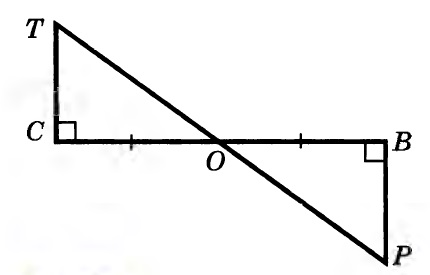
\includegraphics[align=t, width=\linewidth]{../../../../../exercises/lists/pics/G71M7L6-1}
		\end{minipage}
		\item %187
		\begin{minipage}[t]{\bodywidth}
			По данным рисунка докажите, что \(AB \parallel DE\).
		\end{minipage}
		\hspace{0.02\linewidth}
		\begin{minipage}[t]{\picwidth}
			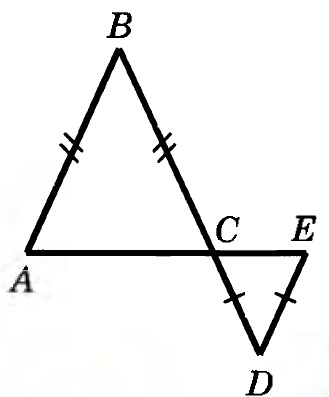
\includegraphics[align=t, width=\linewidth]{../../../../../exercises/lists/pics/G71M7L6-2}
		\end{minipage}
		\item В треугольнике \(ABC\) угол \(A\) равен \(40 \degree\), а угол \(BCE\), смежный с углом \(ABC\), равен \(80 \degree\). Докажите, что биссектриса угла \(BCE\) параллельна \(AB\). %192
		
		%191
		\item Отрезок \(BK\) --- биссектриса треугольника \(ABC\). Через точку \(K\) проведена прямая, пересекающая сторону \(BC\) в точке \(M\) так, что \(BM=MK\). Докажите, что \(KM \parallel AB\). 
		\item На сторонах вертикальных углов отложены от его вершины равные отрезки \(OA, OB, OC\) и \(OD\). Укажите пары равных треугольников с вершинами в точках \(O, A, B, C\) и \(D\).
		%190
		\item 
		\begin{minipage}[t]{\bodywidth}
			На рисунке \(AB=BC, AD=DE, \angle C = 70 \degree, \angle EAC = 35 \degree\). Докажите, что \(DE \parallel AC\)
		\end{minipage}
		\hspace{0.02\linewidth}
		\begin{minipage}[t]{\picwidth}
			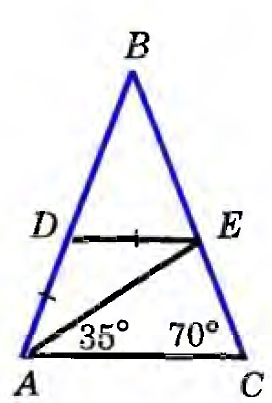
\includegraphics[align=t, width=\linewidth]{../../../../../exercises/lists/pics/G71M7L6-3}
		\end{minipage}
	\end{listofex}
\end{class}
%END_FOLD

%BEGIN_FOLD % ====>>_ Домашняя работа 3 _<<====
\begin{homework}[number=3]
	\begin{listofex}
		\item  Угол \( ABC\) равен \( 70\degree \), а угол \( BCD \) равен \( 110\degree \). Могут ли прямые \( AB \) и \( CD \) быть:
		\begin{tasks}(1)
			\task[a)] параллельными
			\task[б)] пересекающимися?
		\end{tasks}
		\item Периметр равнобедренного треугольника равен \( 1 \) м, а основание равно \( 0,4 \) м найдите длину боковой стороны.
		\item Отрезки \( AC \) и \( BD \) перескекаются в точке \( O \). Докажите равенство треугольников \( BAO \) и \( DCO \), если известно, что угол \( BAO \) равен углу \( DCO \) и \( AO=CO \).
		\item 
		\begin{minipage}[t]{\bodywidth}
			Дано: \\\ \( AC \) ‒ биссектриса \( \angle A \), \( AB=AD \).\\\ Доказать: \( BC = CD \).
		\end{minipage}
		\hspace{0.02\linewidth}
		\begin{minipage}[t]{\picwidth}
			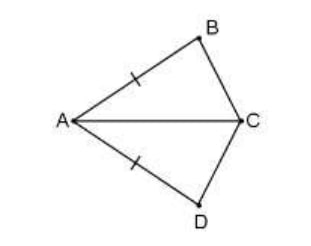
\includegraphics[align=t, width=\linewidth]{../../../../../exercises/lists/pics/sorokinM7H3-1}
		\end{minipage}
		\item На сторонах угла \( BAC \) отложили равные отрезки \( AM \) и \( AN \). На биссектрисе угла \( A \) взяли точку \( D \) и соединили с \( M \) и \( N \). Доказать, что \( DM=DN \).
	\end{listofex}
\end{homework}
%END_FOLD

%BEGIN_FOLD % ====>>_____ Занятие 4 _____<<====
\begin{class}[number=4]
	\begin{listofex}
		\item Пусто
	\end{listofex}
\end{class}
%END_FOLD


%BEGIN_FOLD % ====>>_ Проверочная работа _<<====
\begin{exam}
	\begin{listofex}
		\item Проверочная
	\end{listofex}
\end{exam}
%END_FOLD